\chapter{Introduction}

Since first processors of x86 platform were released big race for who introduce processor with operating on higher frequency started.
This was conditioned to research new production technoligies that allow to integrated more transistors onto smaller area.
In the process manunfacturers started to realize that it is impossible to continue this frequency race forever.
This results integration of more computing units into single processor.
This first among common desktop processors was Intel's \textregistered{Pentium} with hyper threading.
This processors was able to execute two threads at a time.
Since then qick boom of multi core integration started even among other biggest processor manufacturers.
Integration of more execution cores allows less power consumption.
This factor is nowadays especially important due to processor integration into labtops and even due to environmental issues.
Thats why current efforts of processor manufacturers is to gain the best performance to power consumption ratio.

Cores that are ingreated into the current processors are general purpose.
This means thay have pipeline for instruction execution with several stages.
Instruction can be with several states within such pipeline, e.g. fetched, awaiting operands, ready, executed.
Instruction flows among the stages not in the order they are within the program.
Order is decided by the processor based on variety factors and predictions.
One of the pipeline stages is branch prediction unit that has to predict the most probable flow of the executed program.
When this predicion is false whole pipeline has to be discarded and execution of the right branch of program has to be started.
Processors suffer heavily from mispredicions because they lead into big holes in which the processor pipeline stalls or is being reset.

Another general purpose processor suffering is from cache misses.
This occurs when requested data are not within processor cache and have to be load from memory.

Altough many of improvements were implemented into the general purpose processors they still suffer from the described problems.
This is one of the reasons why collaboration of three big companies IBM, Sony, and Toshiba started development of Cell B.E. processor.
Processor that is multicore, has good performance to power consumption ratio and is able to overcome the problems that the general purpose processors suffer.
Because it allow the programmer to somewhat manage processor cache and branch prediction unit.

\chapter{Cell B.E. platform}

This chapter will introduce Cell Broadband Engine processor (Cell B.E.) and the whole platform and its specific details.
Particular Cell B.E. processor will be desribed and illustrated.

\section{About the processor}

Cell B.E. processor is representative of a new generation of IBM's Cell B.E. platform family.
Cell B.E. is an asymmetric, high-performance multi-core processor that combines eight synergistic processing elements (SPEs) and a Power Processing Element (PPE), which is a general-purpose IBM \textregistered{PowerPC} core.
Next part is a central memory element.
PPE can operate with the central memory directly while SPE indirectly, see below.
In Cell B.E. is several kinds memories.
All the elements are connected through high speed bus (EIB - Element Interconnect Bus).
Whole layout is on figure \ref{fg:processorLayout}.

\begin{figure}
    \centering
    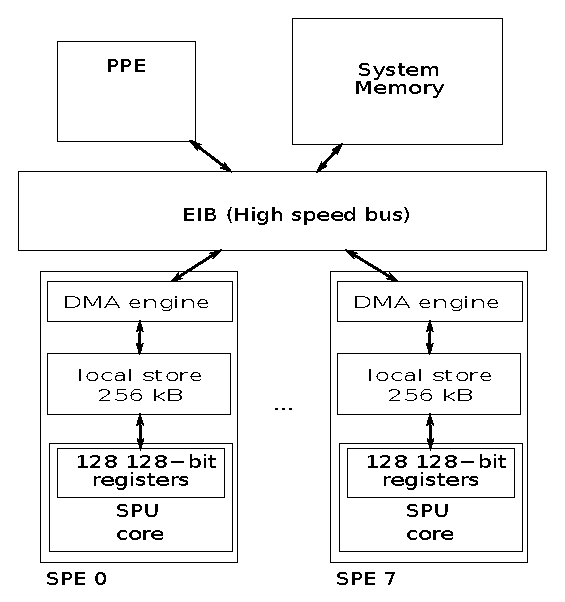
\includegraphics[width=\textwidth]{data/cellLayout}
    \caption[Cell B.E. processor layout]{One PPE unit along with eight SPE stream processor units and system memory connected together with high speed EIB bus}
    \label{fg:processorLayout}
\end{figure}

Each SPE has a 4-way SIMD unit, a high-speed private local store memory and a direct memory access (DMA) engine.
The SIMD unit has 128 128-bit wide general purpose registers.
Vectorized operations in various data types configurations can be performed with these registers.
E.g. two double-precision floats or 8 32bit integers can be processed at single clock tick.
Unlike conventional microprocessors, SPE does not have a hardware cache.
Its function supply the small on-chip local store memory under programmer's control.
This allow code optimizations that can reduce cache misses.
The local store is separated from the main memory (on which the PPE operates), so SPE has its own address space.
Therefore any synchronization with other cores is not necessary.
The local store is attached to a larger (central) shared memory through DMA engine that
manages transfering data from central memory to local store and vice versa.
Therefore, this Cell B.E. can be viewed as a distributed memory multiprocessor.

Cell B.E. achieves a significant performance per Watt and performance per chip area advantage over conventional high-performance processors.
Is significantly more flexible and programmable than single-function and other optimized processors such as graphics processors, or conventional digital signal processors.
While a conventional microprocessor may deliver about 20+GFlops of single-precision (32b) floating-point performance, Cell delivers 200+ GFlops (in ideal conditions) at comparable power.

A number of signal processing and media applications have been implemented on Cell with excellent results.
Advanced visualization such as ray-casting, ray-tracing, and volume rendering.
Streaming applications such as media encoders and decoders and streaming encryption and decryption standards have also been demonstrated to perform about an order of magnitude better on Cell than on conventional PC.

\subsection{PPE - \textregistered{PowerPC} Processing Element}
PPE is derived from IBM \textregistered{PowerPC} core. Has 512kB L2 cache on die.
It supports the Power Architecture ISA, inherits the memory translation, protection, and SMP coherence model of mainstream 64-bit Power processors.
CBEA also supports virtualization (logical partitioning), large pages, and other recent innovations in the Power architecture.
Programming for the PPE is the same as for conventional processors due to direct access to central memory.

\subsection{SPE - Synergistic Processing Element}
SPE is an autonomous processor (sometimes called accelerator) targeted for computational intensive applications.
It supports a SIMD-RISC instruction set.
Has 128 (128-bit long) unified registers to store all types of data (in contrast from traditional RISCs where registers are divided according data types).
One of Cell B.E. programming aspects is converting the code that it uses the SIMD instructions.
This process is called "SIMDation".

SPE stores its program and data in its associated local storage memory as private memory.
DMA transactions are used to transfer data from/to central memory as well as between two local stores.
We say that data is "DMAed" from source to destination.
DMA commands can be issued in many ways.
Synchronous, asynchronous, in scatter-gather manner through DMA lists.
This memory management is another big part of programming for Cell B.E..

Programming for SPE has some differences over programming for conventional processor.
Programmer have always to count with the fact that have only 256kB for the program and data.

This processor is embeded in Sony Playstation 3 game console as well as IBM Blade servers where two or more such processors (as building blocks) connected by high speed bus creates powerfull and modular machine.
We have PlayStation3 machine available for this work.